\section{Variational Autoencoder}\raggedbottom
Variational Autoencoder \citep{kingma2014autoencoding} gehören zu den probabilistischen generativen Modelarchitekturen. In den letzten Jahren haben generative Modelle, insbesondere auch Variational Autoencoder, beeindruckende Möglichkeiten aufgezeigt, um hochrealistische Daten wie zum Beispiel Bilder, Text oder Audios zu generieren.
Generative Modelle versuchen die Merkmale und Verteilung eines Datensatzes zu verstehen und anschließend neuartige Datenbeispiele, die ähnlich zum Trainingsdatensatz sind zu generieren.

Normale Autoencoder bestehen aus einem Encoder und einem Decoder, wobei der Encoder versucht eine komprimierte Darstellung $c\in \mathbb{R}^m$ für die Eingabedaten $x\in \mathbb{R}^n$ im Latentspace zu finden. Die komprimierte Darstellung im Latentspace wird vom Decoder rekonstruiert mit dem Ziel eine möglichst identische Rekonstruktion zur Eingabe $x\in \mathxbb{R}^n$ zu erzeugen.
Autoencoder erzeugen nur einen diskreten Latentraum, wodurch Interpolation durch den Latentraum um neue Ausgaben zu rekonstruieren kaum möglich ist, da im Latentraum viele leere Stellen existieren. Dies ist darauf zurückzuführen, dass ein Autoencoder auf möglichst geringen Verlust beim Encodieren und Decodieren trainiert wird und somit keinen Wert auf die Organisation des Latentspaces legt. Somit entsteht für die einzelnen Datenpunkte ohne Regularisierung oft Overfitting.

Im Gegensatz zu normalen Autoencodern verwenden Variational Autoencoder einen probabilistischen Ansatz um Datenpunkte $x$ im Latentspace $Z$ zu repräsentieren. 
Der Encoder des Variational Autoencoder encodiert die Eingabe in eine multivariate Verteilung von der die Latentvektoren gesamplet werden. Die Latentvektoren werden anschließend vom Decoder decodiert und der Rekonstruktionserror zurückgegeben.
%Normalerweise werden für die Encodierteverteilung 
%Normalverteilung Regalusierung erklären https://towardsdatascience.com/understanding-variational-autoencoders-vaes-f70510919f73

\begin{figure}[h]
    \centering
    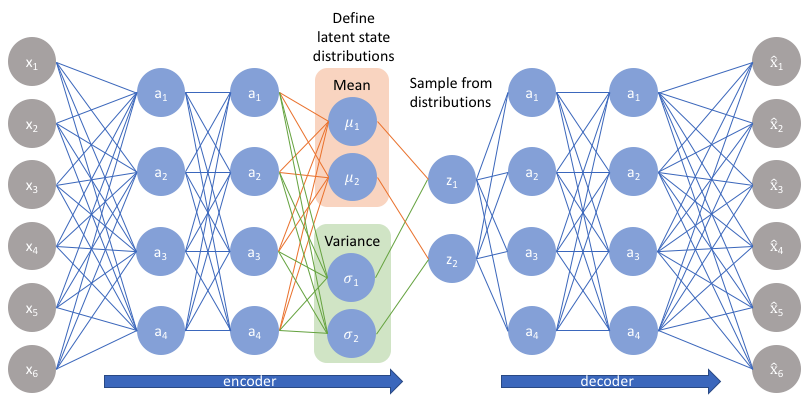
\includegraphics[width=11cm]{bilder/vae}
    \caption{VAE Modellarchitektur}
    \label{vae_model}
\end{figure}
Die Beziehungen zwischen den Eingabedaten $x$ und den Latentvektoren $z$ sind wie folgt definiert, wobei $\phi$ die Parameter des Encoders und $\theta$ die Parameter des Decoders sind:
\begin{itemize}
\item Prior $p_\theta (z)$
\item Likelihood $p_\theta (x|z)$
\item Posterior $p_\theta (z|x)  \approx q_\phi (z|x)$
\end{itemize}

Da die Posterior Verteilung $p_\theta (z|x)$ nicht bestimmt werden kann approximieren wir diese mit $q_\phi (z|x)$ unter Verwendung der Variationsinferenzmethode zur Minimierung der Kullback-Leibler-Divergenz, wie in Abschnitt \ref{elbo} beschrieben.

Um mittels Variational Autoencoder neue Datenobjekte zu samplen wird zunächst mit der Prior-Verteilung $p_\theta (z)$ ein neuer Latentvektor $\hat{z}$ gezogen. Anschließend lässt sich ein neues Datenobjekt $\hat{x}$ mit der Verteilung $p_\theta (x|z=\hat{z})$ generieren.
\subsection{Evidence Lower Bound}
%https://lilianweng.github.io/lil-log/2018/08/12/from-autoencoder-to-beta-vae.html#contractive-autoencoder
%https://openreview.net/forum?id=Sy2fzU9gl
%https://arxiv.org/pdf/1312.6114.pdf
%http://mediatum.ub.tum.de/doc/1547089/1547089.pdf
%https://pub.tik.ee.ethz.ch/students/2018-FS/MA-2018-22.pdf
%https://mediatum.ub.tum.de/doc/1547089/file.pdf
%https://www.jeremyjordan.me/variational-autoencoders/
%https://towardsdatascience.com/understanding-variational-autoencoders-vaes-f70510919f73
%https://arxiv.org/pdf/1906.02691.pdf
%https://arxiv.org/pdf/1903.10145.pdf
%https://ichi.pro/de/generative-modellierung-mit-variational-auto-encoder-vae-277371603749134
%https://xyang35.github.io/2017/04/14/variational-lower-bound/

\label{elbo}
Bei Variational Autoencodern ist das Optimierungsziel die Minimierung des Rekonstruktionsfehlers zwischen Eingabe- und Ausgabedaten und die Approximation von $p_\theta (z|x)$ durch Minimierung der Kullback-Leibler-Divergenz $D_{KL}(q_\phi (z|x) \parallel p_\theta (z|x) )$.
\begin{align*}
    \small
    D_{KL}(q_\Phi(\mathbf{z\mid x})\parallel p_\theta(\mathbf{z\mid x})) &= \int q_\Phi(\mathbf{z\mid x}) \log \frac{q_\Phi(\mathbf{z\mid x})}{p_\theta(\mathbf{z\mid x})} \, d\mathbf{z}\\
    &= \int q_\Phi(\mathbf{z\mid x}) \log \frac{q_\Phi(\mathbf{z\mid x})p_\theta(\mathbf{x})}{p_\theta(\mathbf{z,x})} \,d\mathbf{z}\\
    &= \int q_\Phi(\mathbf{z\mid x}) \left( \log (p_\theta(\mathbf{x})) + \log \frac{q_\Phi(\mathbf{z\mid x})}{p_\theta(\mathbf{z,x})}\right) d\mathbf{z}\\
    &= \log (p_\theta(\mathbf{x})) + \int q_\Phi(\mathbf{z\mid x}) \log \frac{q_\Phi(\mathbf{z\mid x})}{p_\theta(\mathbf{z,x})} \,d\mathbf{z}\\
    &= \log (p_\theta(\mathbf{x})) + \int q_\Phi(\mathbf{z\mid x}) \log \frac{q_\Phi(\mathbf{z\mid x})}{p_\theta(\mathbf{x\mid z})p_\theta(\mathbf{z})} \,d\mathbf{z}\\
    &= \log (p_\theta(\mathbf{x})) + E_{\mathbf{z} \sim q_\Phi(\mathbf{z\mid x})}(\log \frac{q_\Phi(\mathbf{z\mid x})}{p_\theta(\mathbf{z})} - \log(p_\theta(\mathbf{x\mid z})))\\
    &= \log (p_\theta(\mathbf{x})) + D_{KL}(q_\Phi(\mathbf{z\mid x}) \parallel p_\theta(\mathbf{z})) - E_{\mathbf{z} \sim q_\Phi(\mathbf{z\mid x})}(\log(p_\theta(\mathbf{x\mid z})))
    \end{align*}
der \textbf{E}vidence \textbf{L}ower \textbf{B}ound (ELBO).


ÜBERARBEITEN
\subsubsection{Reparametisierung} %kingma welling
Zum Training des Variational Autoencoder wird mittels Backpropagation der Fehler des Netzwerkes propagiert. Da das Samplen von $z /sim q_\Phi(z|x)$ nicht deterministisch ist, kann hier keine Backpropagation durchgeführt werden.
Um dennoch Backpropagation verwenden zu können wird durch Reparametisierung $z$ durch eine deterministische Funktion $z=f_\Phi(x,\epsilon)$ dargestellt mit $\epsilon$ als externe unabhängig zufällige Hilfsvariable. 
Bei einer multivariaten Gaussverteilung für $q_\Phi (z|x)$ wäre die Reparametisierung wie folgt, wobei $\times$ die elementweise Multiplikation denotiert:
\begin{align}{}
    z \zim q_\Phi(z|x) = \mathcal{N}(z;\mu,\sigma \mathcal{I}) \\
    z = \mu + \sigma \times \epsilon \text{ , mit } \epsilon \sim \mathcal{N}(0,\mathcal{I}) 
\end{align}

\subsection{Cyclical Annealing Schedule}
\label{cyc_anneal}
Trainieren von Variational Autoencodern als Sprachmodell im Bereich des Natural Language Processing ist aufgrund des KL-Vanishing Problems besonders schwierig.
VAE Sprachmodelle sollen bei der Textgeneration den lokalen Kontext, allerdings auch globale Eigenschaften wie zum Beispiel Thema, Sprachstil oder Stimmung beachten. 
Trotzdem werden von VAE Modellen bei der Generation oft die globalen Eigenschaften vernachlässigt. 
Dieses Problem ist als KL-Vanishing bekannt, da die KL-Regularisierung des Loss Terms beim Trainieren von autoregressiven Decodern innerhalb von VAE Sprachmodellen sehr klein wird.
Somit sind die erlernten Features nahezu identisch zu der vorher angenommenen Normalverteilung und der Decoder nutzt keine Latentfeatures. %https://www.microsoft.com/en-us/research/blog/less-pain-more-gain-a-simple-method-for-vae-training-with-less-of-that-kl-vanishing-agony/ nochmal checken

Abhilfe schafft die Verwendung eines $\beta$-Variational Autoencoder mit zyklischem erhöhen des $\beta$ Wertes.
$\beta$-Variational Autoencoder sind Variational Autoencoder die mit einen Lagrangemultiplikator $\beta$ die KL-Divergenz der Loss-Funktion gewichten um besser separierte Latentfaktoren zu finden.
\begin{equation}
    L_{\beta}(\Phi,\theta,\beta) = -\mathbb{E}_{z\sim q_\Phi(\mathbf{z\mid x})}[log p_\theta (\mathbf{x\mid z})]- \beta D_{KL}(q_\Phi(\mathbf{z\mid x}) \parallel p_\theta(\mathbf{z})) 
\end{equation}
Falls $\beta = 0$ ist wird das Modell wie ein normaler Autoencoder trainiert, bei $\beta = 1$ wie ein normaler Varitional Autoencoder.

Beim Zyklischen Erhöhen wird der $\beta$-Wert des VAE geplant während des Trainings monoton von $\beta=0$ auf zum Ende des Trainings $\beta=1$ in kleinen Abständen erhöht.
So kann beim Training des VAE bei $\beta<1$ zunächst der Fokus darauf gelegt werden mehr Information für die Rekonstruktion zu erlernen. 
Abschließend enthalten bei $\beta=1$ die bereits vorher trainierten $z$ Vektoren bereits mehr Informationen die zu einer besseren Anpassung als eine zufällige Initialisierung führen.




\subsection{Optimus}
Optimus (\textbf{O}rganizing \textbf{S}entences via \textbf{P}re-trained \textbf{M}odeling of a \textbf{L}atent \textbf{S}pace) \citep{DBLP:journals/corr/abs-2004-04092} ist ein großes vortrainiertes Deep Latent Variable Model für natürliche Sprache.
Die Modelarchitektur von Optimus ist ein Variational Autoencoder, der als Encoder BERT und als Decoder GPT-2 verwendet wie in Abbildung \ref{optimus_scheme_fig} zu erkennen ist. 
Verwendet wird jeweils das vortrainierte BERT Base Modell $\phi_{BERT}$ und das vortrainierte GPT-2 Base Modell $\theta_{GPT-2}$ beide mit 12 Layern, 12 Attention Heads und einer Hiddensize von 768. 
\begin{figure}[h]
    \centering
    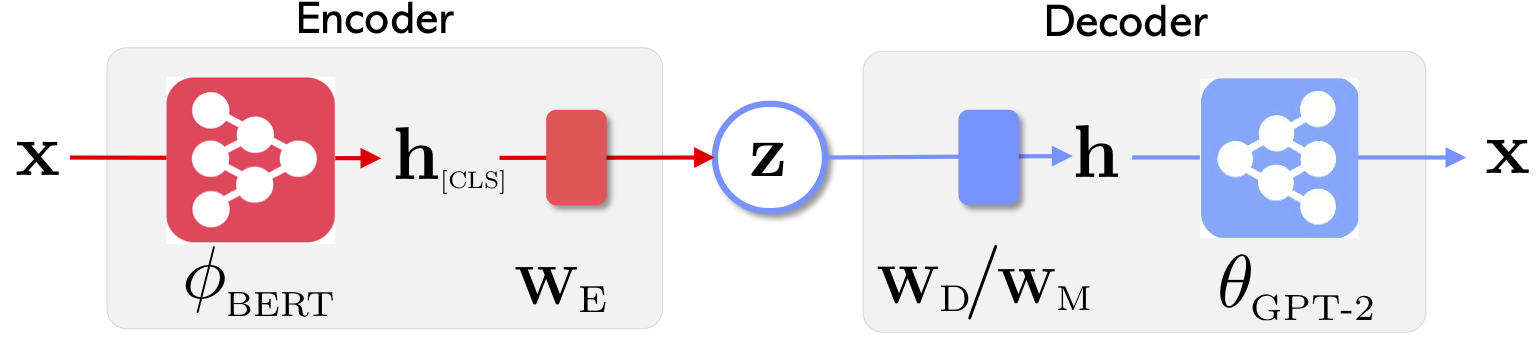
\includegraphics[width=\textwidth]{bilder/optimus_scheme}
    \caption{VAE Modellarchitektur von OPTIMUS mit BERT als Encoder und GPT-2 als Decoder}
    \label{optimus_scheme_fig}
\end{figure}
Trainiert wird Optimus mit dem Ziel Sätze in einen universellen Latentspace zu organisieren und somit übergreifende semantische Muster für die einzelnen Sätze zu finden.
Somit kann durch gezieltes Verändern des Latentvektors $z$ kontrolliert Text generiert werden. ÜBERARBEITEN

BERT und GPT-2 über eine VAE Architektur miteinander zu verbinden hat die Herausforderung die unterschiedlichen Tokenisierungsschemen der einzelnen Modelle zu verwenden und den Latentvektor bei der Textgeneration von GPT-2 zu injizieren. 
Die Eingabetokens von BERT verwenden das WordPiece Embeddings verfahren mit einer Vokabulargröße von 28.996. Die Ausgabe erfolge über die Byte Pair Encoding Tokenisierung von GPT-2 mit einer Vokabulargröße von 50.260. Innerhalb des Netzwerkes wird im Latentvektor ein Token durch eine Einbettung $h_{Emb}$ die das Token, die Position und das Segment Embedding wiedergibt, repräsentiert.
Um beim Training den Loss des Rekonstruktionstask zu berechnen, werden die Sätze mit beiden Tokenisierungen tokenisiert.

Als Latentvektor $z \in \mathbb{R}^P$ wird die gepoolte Ausgabe des letzten Hiddenlayers $h_{[CLS]} \in \mathbb{R}^H$ von BERT multipliziert mit einer Gewichtsmatrix $W_{E} \in \mathbb{R}^{P\times H}$ gewählt. Somit kann ein Latentvektor wie folgt bestimmt werden $z = W_{E}h_{[CLS]}$.

\begin{figure}[h]
    \centering
    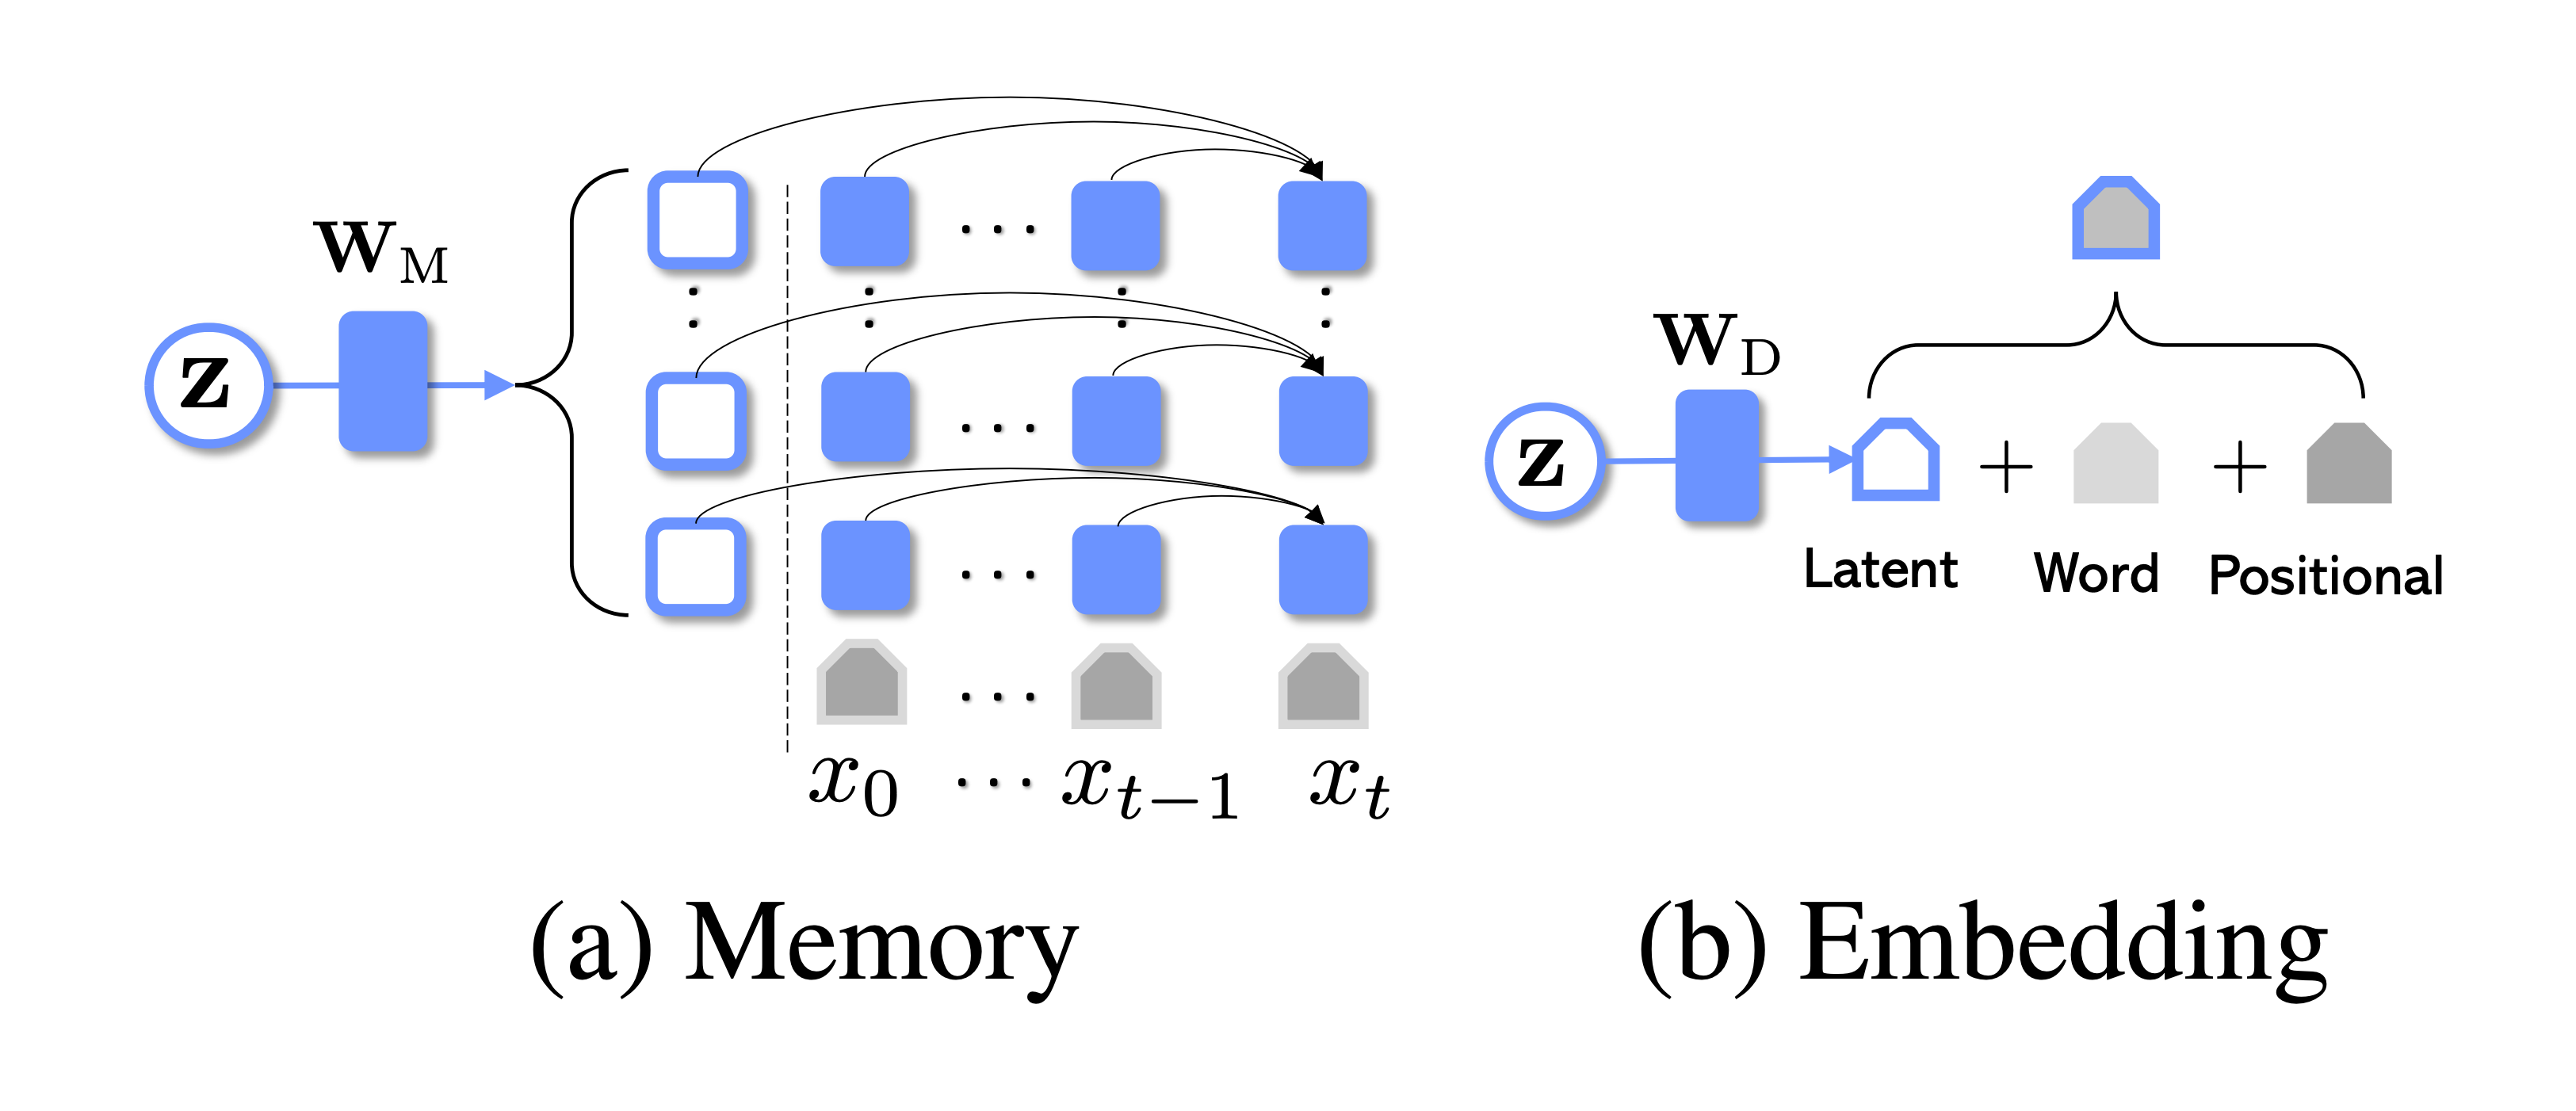
\includegraphics[width=8cm]{bilder/latent_optimus}
    \caption{Methoden um den Latentvector in GPT-2 zu injizieren}
    \label{latent_optimus}
\end{figure}

Um mit GPT-2 kontrolliert unter Verwendung des Latentvektors Text zu generieren kann der Latentvektor entweder als Memoryvektor in die Past-Gewichtsmatrix injeziert oder auf die alten Embeddings addiert werden.

Beim Embedding wird $z$ direkt auf den Embedding Layer addiert. Somit ergibt sich der neue Embedding Layer durch $h_{Emb}^{'} = h_{Emb} + W_D z$ mit der Gewichtsmatrix $W_D \in \mathbb{R}^{H \times P}$.
Der Decoder kann hier die zusätzlichen Informationen des Embeddings beim Input und Output Layer verwenden.

Bei der Injezierung von $z$ als Memoryvektor $h_{Mem} \in \mathbb{R}^{L\times H}$ wird der Latentvektor in den Past Key Vektor von GPT-2 injeziert. Der Past Key Vector beschleunigt normalerweise den Decodiervorgang von GPT-2, da bei einem Decodierungsdurchlauf zu den vorherigen Tokens bereits entsprechende Key- und Valuevektoren in den Attentionlayern berechnet wurden.
Diese Key-, Valuevektoren des Attentionlayers werden durch $h_{Mem} = W_M z$ mit $W_M \in \mathbb{R}^{LH \times P}$ ersetzt. GPT-2 kann so beim Decodieren auf den injezierten Latentvektor bei jeder Attentionberechnung zugreifen.

Die Parameter ${\phi_{BERT}, \theta_{GPT-2}, W_E,W_M,W_D}$ des VAEs werden mittels Cyclical Annealing Schedule \citep{DBLP:journals/corr/abs-1903-10145} trainiert, um das KL Vanishing Problem beim Trainieren eines VAEs zu verhindern.
Die $\beta$ Variable, die wie in \ref{cyc_anneal} erklärt den KL Regularisierer Anteil steuert, wird für einen Trainingsdurchlauf für die erste halbe Menge der Trainingsdaten auf $\beta = 0$ gesetzt. Somit wird zu Beginn lediglich ein Autoencoder trainiert. 
Anschließend wird für das nächste viertel der Trainingsmenge schrittweise $\beta$ von 0 auf 1 erhöht und für das letzte viertel der Trainingsmenge auf 1 belassen um das VAE Model zu trainieren.

Insgesamt zeigt Optimus gute Ergebnisse in den Bereichen des Language Modeling, Kontrollierte Text Generation und Language Understanding.




\subsection{Latent Space Operations}

\pagebreak
